\clearpage
\subsection{Type Declaration} % (fold)
\label{sub:type_declaration}

Type declarations allow you to define your own types. Programming Languages offer a range of different code structures you can use to build your own types.

\begin{figure}[h]
   \centering
   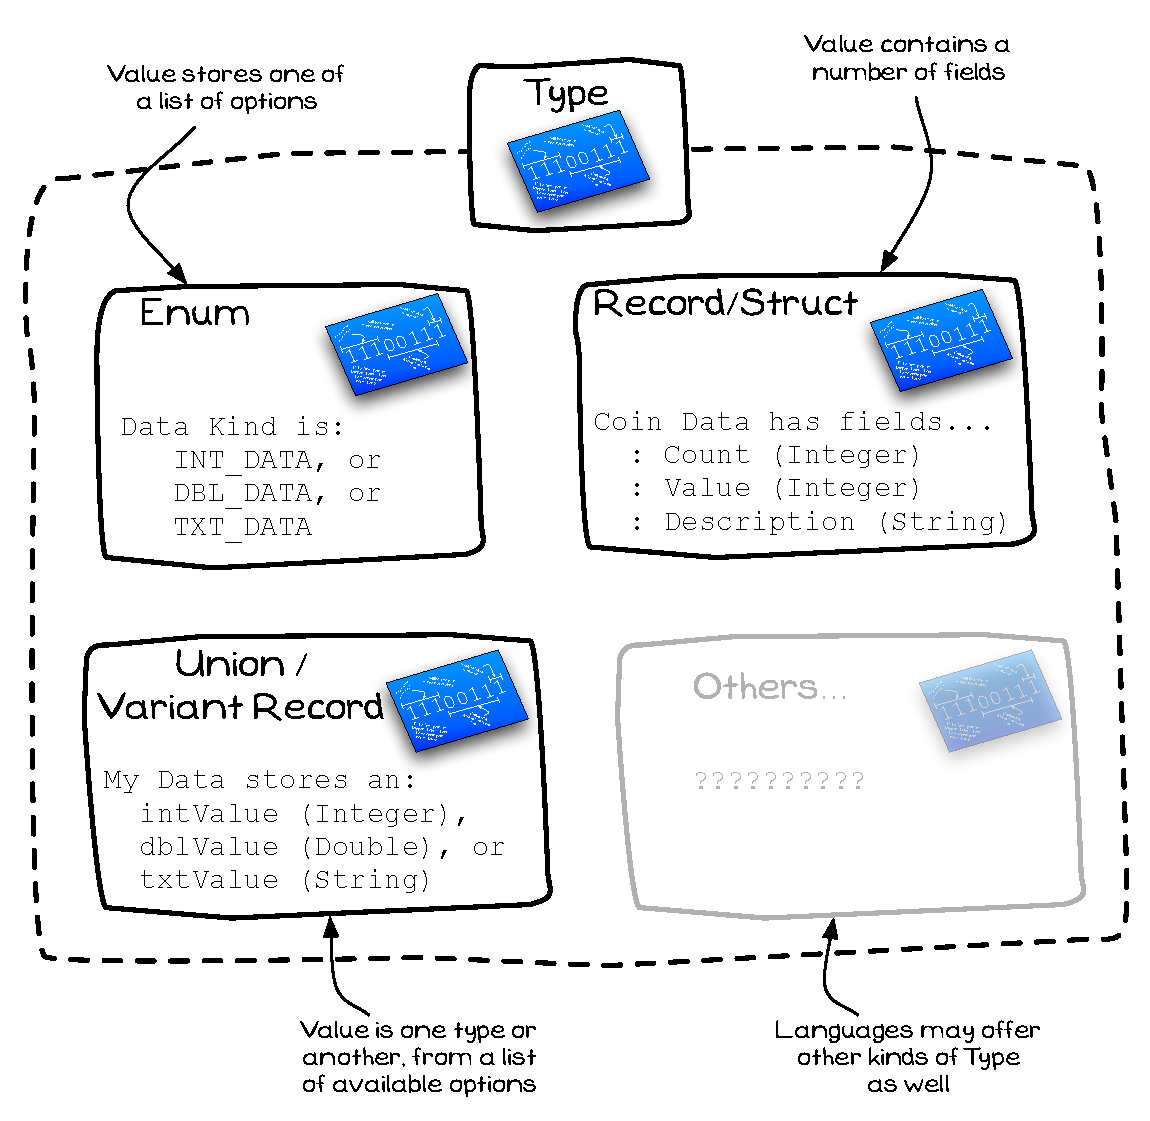
\includegraphics[width=0.9\textwidth]{./topics/type-decl/diagrams/TypeDecl} 
   \caption{You can declare your own Data Types}
   \label{fig:type-decl-type-decl}
\end{figure}

\mynote{
\begin{itemize}
  \item A type declaration is the \textbf{term} given for declaring your own type \emph{artefact} in code.
  \item Programming Languages offer a range of different kinds of types that you can create.
  \item Each kind of type declaration allows you to create a type for different kinds of values:
  \begin{itemize}
    \item \textbf{Enum}: An enumeration is creates a type where the value will be one of a list of available options.
    \item \textbf{Record} or \textbf{Struct}: A structured record, where each value of this type is made up of a number of fields.
    \item \textbf{Union} or \textbf{Variant Record}: Makes it possible to create a type where the value could be one of a number of other types.
    \item Languages may also offer other kinds of type you can declare.
  \end{itemize}
  \item You use these different kind of types to design the structure for the values you will work with in your code.
  \item There is no data associated with a type declaration, you are declaring a new format, not another value.
\end{itemize}
}

\clearpage
\subsection{Record or Structure} % (fold)
\label{sub:record_or_structure}

\begin{figure}[h]
   \centering
   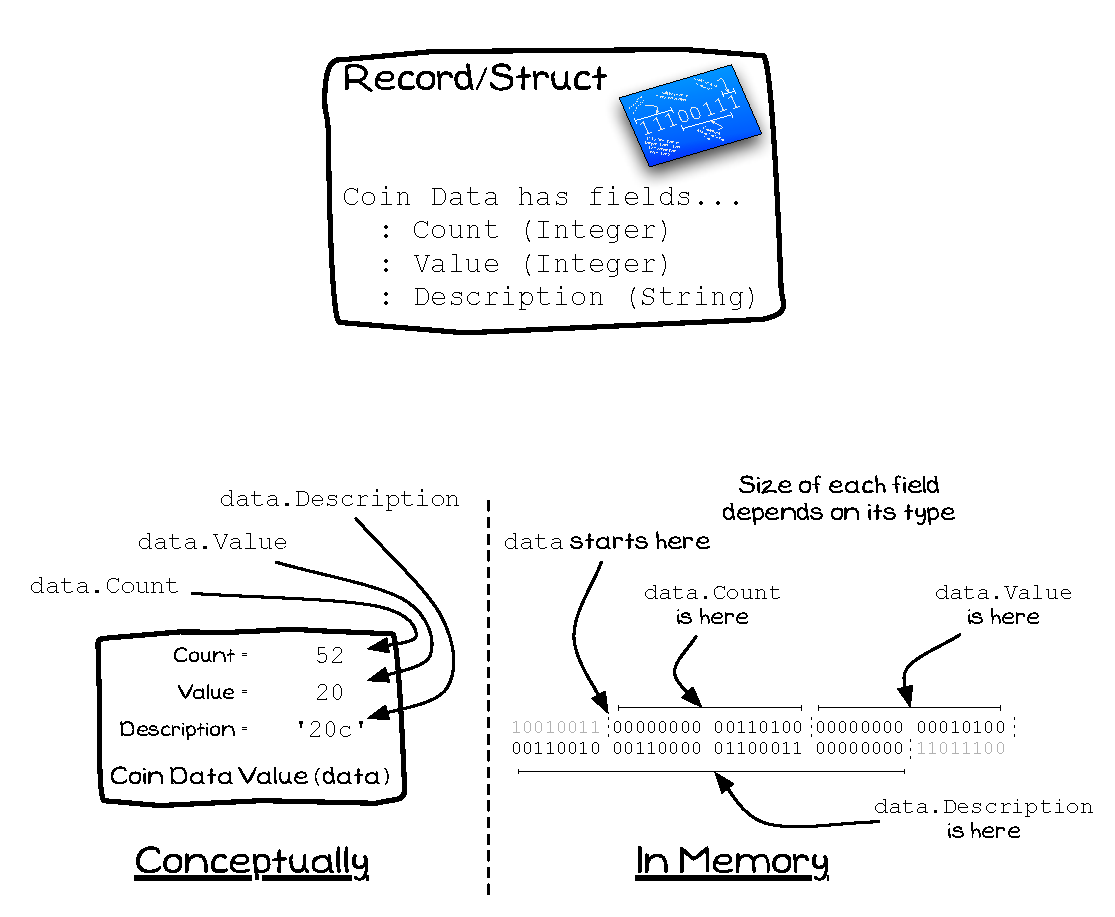
\includegraphics[width=\textwidth]{./topics/type-decl/diagrams/Record} 
   \caption{A Record or Structure contains Fields}
   \label{fig:type-decl-record}
\end{figure}

% subsection record_or_structure (end)
\clearpage
\subsubsection{Enumeration} % (fold)
\label{ssub:enum}

An Enumeration allows you to create a type where the value is one of a list of available options. When you declare an enumeration you are listing the values that are available for data of this type. The example in \fref{fig:type-decl-enum} declares a type that can have the value \texttt{ADD\_COINS} or \texttt{REMOVE\_COINS}.

\begin{figure}[h]
   \centering
   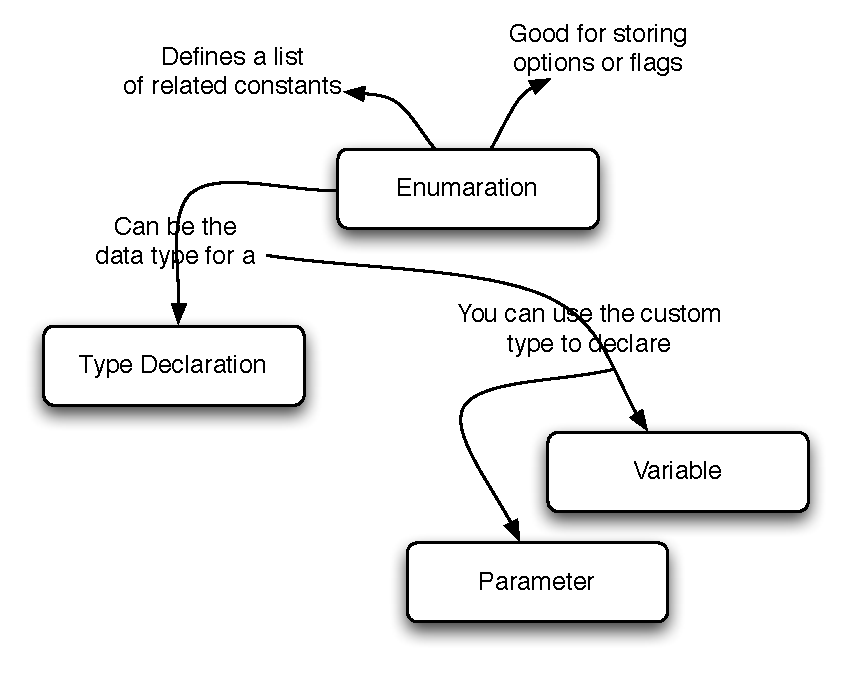
\includegraphics[width=\textwidth]{./topics/type-decl/diagrams/Enum} 
   \caption{An Enumeration allows you to define related constants}
   \label{fig:type-decl-enum}
\end{figure}

\mynote{
\begin{itemize}
  \item An Enumeration is a kind of \textbf{artefact} that you can declare.
  \item Using an enumeration you can declare a kind of value that must come from a list of available options.
  \item When you declare the enumeration you list the \emph{values} that it may have.
  \item This is like a list of constants, where values of this type will match one of these constants.
  \item Internally the compiler will map your values to numeric values. The first option is represented by the value \texttt{0}, the second is represented by the value \texttt{1}, and so on.
  \item You can specify the values for each option in the enumeration, this can be useful if you want to be able to combine options in a single value. In these cases you give each option a bit unique value (first at \texttt{1}, then \texttt{2}, \texttt{4}, \texttt{8}, \texttt{16}, etc).
  \item The \textbf{size} of an enumeration is based on the size of the integer type used to represent its values.
\end{itemize}
}

% subsection enumerations (end)
\clearpage
\subsubsection{Union} % (fold)
\label{ssub:union}

A Union (Variant Record in Pascal) allows you to declare a type where the values may be one of a range of alternative types. In effect, you can declare a type where the value may be one of a number of different types. This is useful if you want to store different types of values at a location in your program.

A Union often works best by accompanying it with a \textbf{tag} value. This value then records the kind of data currently being stored at the location in memory. A good option is to use an \nameref{sub:enum} for the tag's type, giving you a range of value, that describe the range of types stored.

\begin{figure}[h]
   \centering
   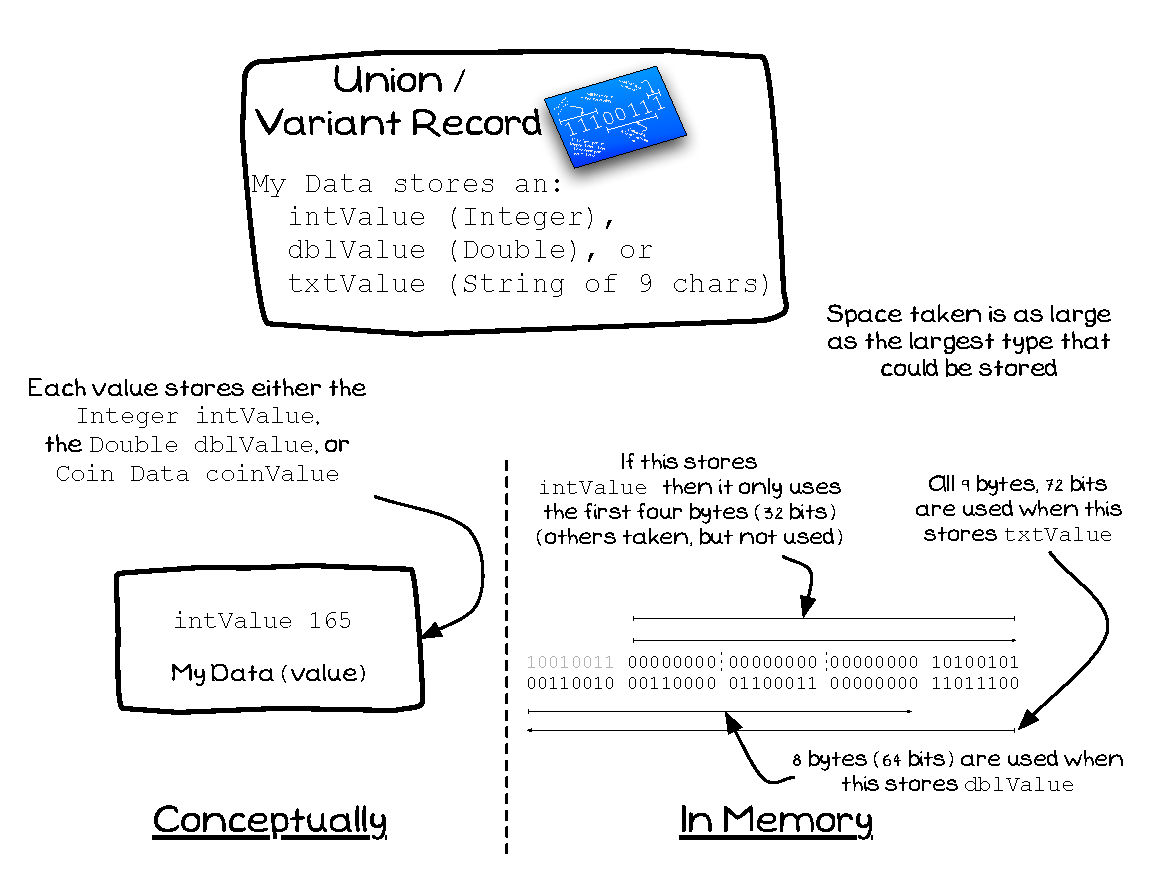
\includegraphics[width=\textwidth]{./topics/type-decl/diagrams/Union} 
   \caption{A Union is one type that can store one of a range of other types}
   \label{fig:type-decl-union}
\end{figure}

\mynote{
\begin{itemize}
  \item A Union is a kind of \texttt{artefact} that you can declare. 
  \item The Union allows you to use one location in memory to store one of a number of types of value.
  \item At any one time this data can be used to store \textbf{one} of these values.
  \item It is the developers responsibility to ensure they access the right kind of value when it is being used.
  \item A \textbf{tag} value can be used to store a marker that indicates the type of data being stored in the union.
  \item The \textbf{size} of a union is the size of its \emph{largest} option. For example a union of a \texttt{Character} (1 byte), a \texttt{Integer} (4 bytes), and a \texttt{Double} (4 bytes) is 4 bytes, the size of the largest kind of value it needs to store.
\end{itemize}
}

% subsubsection union (end)

% subsection type_declaration (end)